% Source: Code/yolo-ablation-bench/unified_report.tex

\documentclass[border=4pt]{standalone}
\usepackage{amssymb}
\usepackage[T1]{fontenc}
\usepackage{graphicx}
\usepackage{helvet}
\usepackage{lmodern}
\usepackage{pgfplots}
\usepackage{pgfplotstable}
\usepackage{tikz}
\usepackage[dvipsnames,table]{xcolor}
\pgfplotsset{compat=1.18}

\definecolor{garnet}{HTML}{73000A}
\definecolor{midgray}{gray}{0.35}
\definecolor{lightgray}{gray}{0.8}
\definecolor{dlacolor}{HTML}{2E7D32}
\definecolor{gpucolor}{HTML}{1565C0}


\newcommand{\headline}[1]{\textcolor{garnet}{\Large\bfseries #1}}
\newcommand{\subhead}[1]{\textcolor{midgray}{\large #1}}
\newcommand{\dla}[1]{\textcolor{dlacolor}{\textbf{#1}}}
\newcommand{\gpu}[1]{\textcolor{gpucolor}{\textbf{#1}}}

\begin{document}
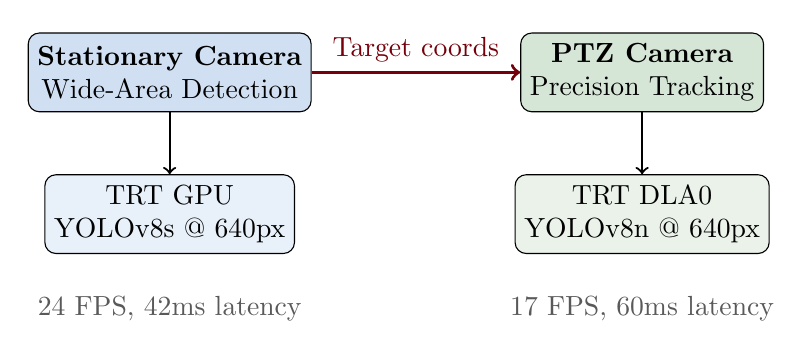
\begin{tikzpicture}[
  box/.style={draw, rounded corners, minimum width=3cm, minimum height=1cm, align=center},
  arrow/.style={->, thick}
]
  % Stationary camera
  \node[box, fill=gpucolor!20] (stat) at (0,0) {\textbf{Stationary Camera}\\Wide-Area Detection};
  \node[box, fill=gpucolor!10] (gpu) at (0,-1.8) {TRT GPU\\YOLOv8s @ 640px};
  
  % PTZ camera
  \node[box, fill=dlacolor!20] (ptz) at (6,0) {\textbf{PTZ Camera}\\Precision Tracking};
  \node[box, fill=dlacolor!10] (dla) at (6,-1.8) {TRT DLA0\\YOLOv8n @ 640px};
  
  % Connection
  \draw[arrow, garnet, very thick] (stat) -- node[above] {Target coords} (ptz);
  \draw[arrow] (stat) -- (gpu);
  \draw[arrow] (ptz) -- (dla);
  
  % Labels
  \node[midgray] at (0,-3) {24 FPS, 42ms latency};
  \node[midgray] at (6,-3) {17 FPS, 60ms latency};
\end{tikzpicture}
\end{document}
